%-------------------------------------------------------------------
% bachelor thesis
%
% topic: ACDC4JS - How to analyze a JavaScript garbage collector
%
% create by: Mario Preishuber
% create date: 2014, Jan 01.
%-------------------------------------------------------------------

\chapter{ACDC4JS}

\section{Preparation}
	For developing a tool like ACDC4JS it is necessary to get some information before starting with implementing. Especially in this case, a lot of information about the structure of typical JavaScript heap had to be collected. The figure \ref{fig:heap_structure_analysis} on page \pageref{fig:heap_structure_analysis} shows the toolchain used to analysis the structure of real JavaScript applications. For the simulation of realistic user interaction on an web page the tool called \texttt{AutomatedUserInteraction} (see section \ref{sec:automated_user_interaction}) is used in combination with a custom version of Chromium. The custom Chromium version produces periodic a snapshot of the heap (for details see section \ref{sec:custom_chromium}). These snapshots are analyzed by the so-called \texttt{HeapSnapshotAnalyzer} (see section \ref{sec:heap_snapshot_analyzer}). The \texttt{HeapSnapshotAnalyzer} used for the analysis an PostgreSQL database in version 9.3 \cite{PSQL13}

	\begin{figure}
		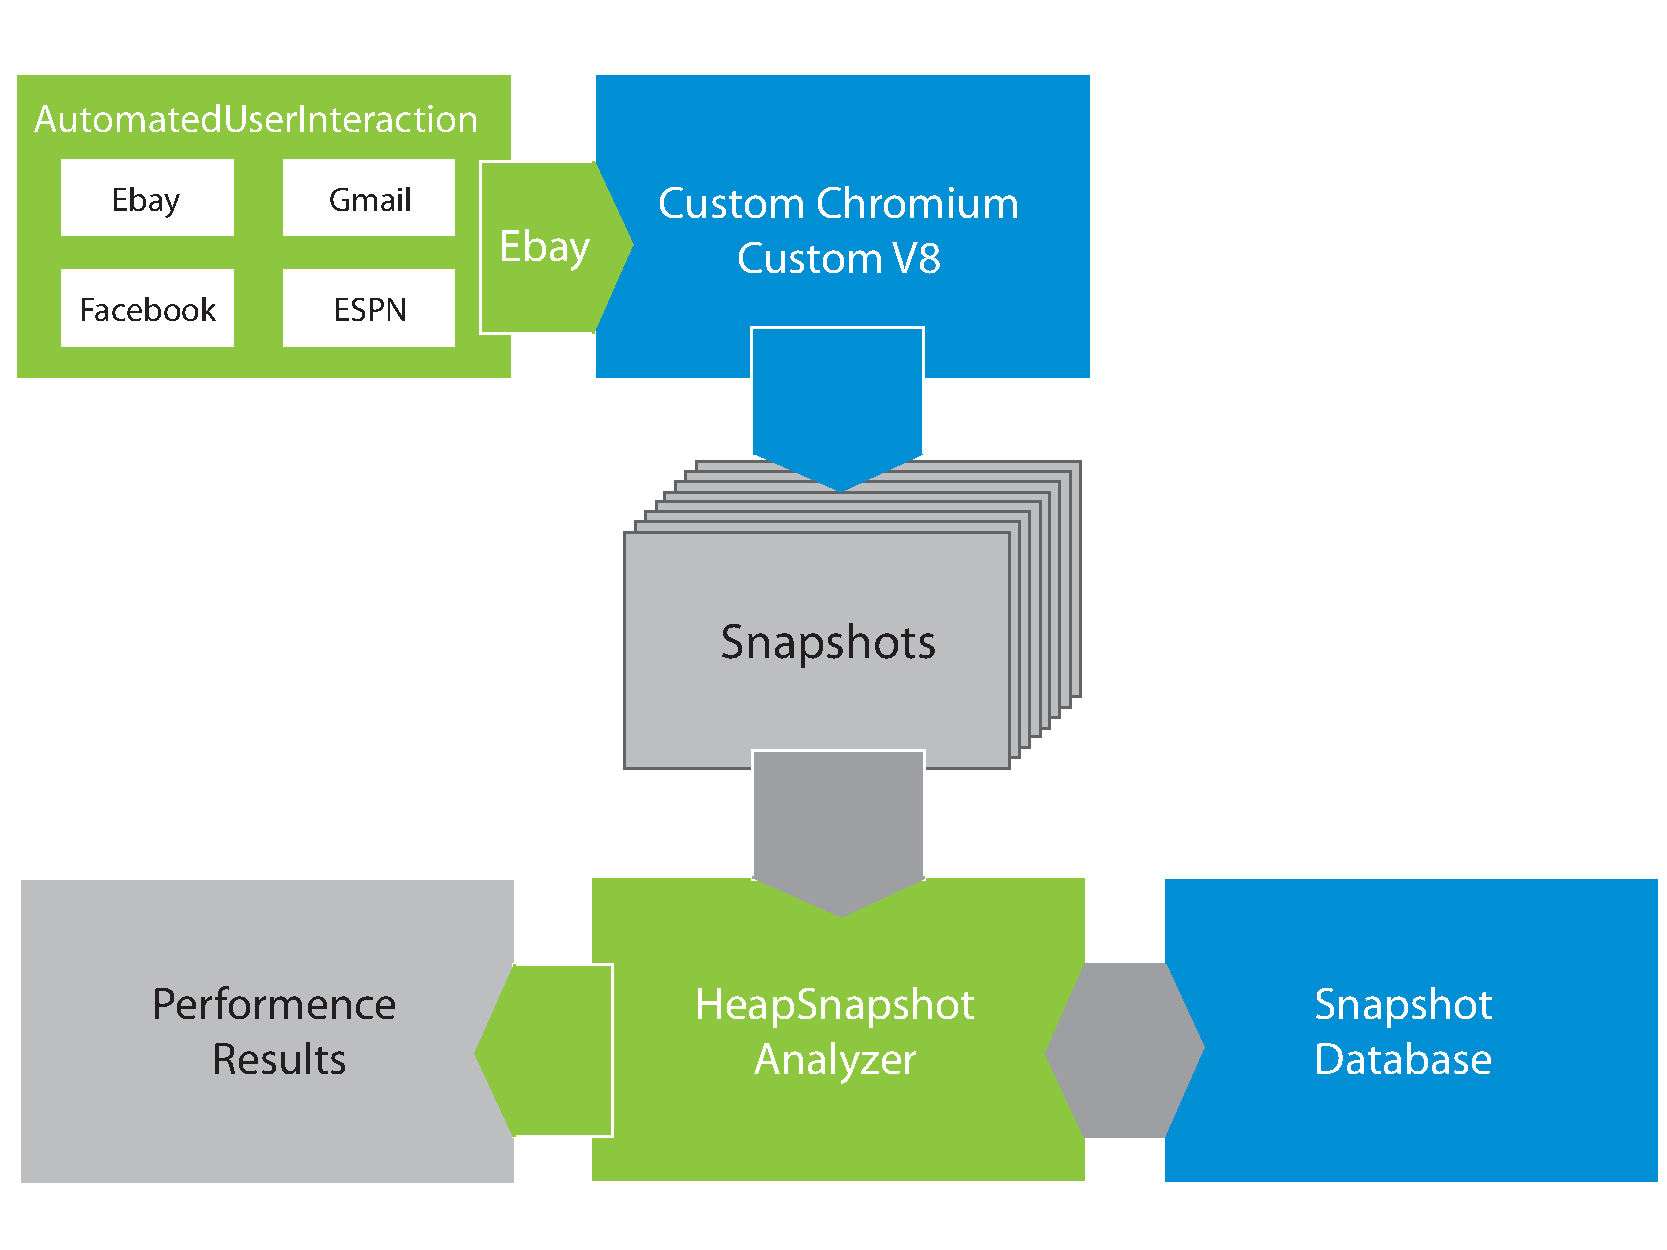
\includegraphics[width=0.7\textwidth]{solution_h.pdf}
		\caption{Tool chain to analyze the JavaScript heap structure of a real web application}
		\label{fig:heap_structure_analysis}
	\end{figure}

	\subsection{AutomatedUserInteraction} \label{sec:automated_user_interaction}
	\subsection{Custom Chromium} \label{sec:custom_chromium}
	\subsection{HeapSnapshotAnalyzer} \label{sec:heap_snapshot_analyzer}

